\documentclass[a4paper]{article}

% page layout and formatting
\usepackage[top=1in,bottom=1in,left=1.2in,right=1.2in]{geometry}
\usepackage{parskip}
\usepackage[small]{titlesec}
\usepackage{amsmath}
\usepackage{color}
\usepackage{graphicx}
\usepackage{hyperref}

% code
\usepackage{minted}
\newenvironment{code}{\captionsetup{type=listing}}

% custom commands
\newcommand{\todo}[1]{\textcolor{red}{\textbf{TODO:} #1}}

% metadata
\title{CS4395 Assignment 2 \\ \begin{small}\url{https://github.com/adibarra/hlt}\end{small}}
\author{Alec Ibarra \\ adi220000}
\date{}

\begin{document}
\maketitle


\section{Introduction and Dataset}

In this report, we implemented and compared two neural network architectures for sentiment classification of Yelp reviews: a Feedforward Neural Network (FFNN) and a Recurrent Neural Network (RNN). The task is a 5-class sentiment classification problem, with sentiment labels from 1 (very negative) to 5 (very positive).

Our experiments involved building models using PyTorch, training them on the provided Yelp dataset, and evaluating their performance based on accuracy and loss. The FFNN uses a bag-of-words representation, while the RNN uses word embeddings and processes the sequence of words in the review.


\subsection*{Dataset Statistics}
The dataset is split into the following sets:

\begin{table}[H]
\centering
\begin{tabular}{|l|c|}
\hline
\textbf{Split} & \textbf{Number of Reviews} \\
\hline
Training Set & 16,000 \\
Validation Set & 800 \\
Test Set & 800 \\
\hline
\end{tabular}
\caption{Dataset statistics for Yelp sentiment classification.}
\label{tab:dataset}
\end{table}

Reviews are preprocessed via tokenization, lowercasing, and index mapping based on the training vocabulary. In the RNN, we use pre-trained word embeddings to initialize word vectors, while the FFNN uses bag-of-words vectors. The dataset has a balanced label distribution.


\section{Implementations}

The models share key implementation elements. Both use the \texttt{Adam} optimizer and the \\\texttt{ReduceLROnPlateau} scheduler, which adjusts learning rates based on performance to aid convergence. They also include early stopping with patience, which halts training if combined training and validation accuracy stagnates over several epochs. Though the training approach is similar, primary differences between the two lie in their architecture.

Both designs balance expressiveness and generalization, using simple yet effective architectures tailored to their inputs. Regularization techniques like dropout help prevent overfitting, while shallow networks and efficient training promote robust generalization. These choices emphasize stability, convergence, and generalization.

The implementations are almost entirely custom, with lots of refactoring to improve efficiency and eliminate deprecated functions. Refactoring also enabled GPU/CUDA support for faster training. Common tasks such as data loading, vectorization, and vocabulary management are centralized in \texttt{utils.py}, simplifying reuse and maintenance.


\subsection*{Dependencies}
The dependencies required to run the models are minimal and were provided as part of the initial starter package. They are listed in the \texttt{requirements.txt} file and include \texttt{numpy}, \texttt{torch}, and \texttt{tqdm}.


\subsection*{Debugging and Resources}
During the implementation process, we encountered several challenges, including deprecated functions, tensor shape mismatches, and the need for efficient data handling. To resolve these issues, we relied heavily on the official PyTorch documentation, which helped us identify correct usage patterns and appropriate alternatives to outdated APIs.

We also referred to tutorials on deep learning with PyTorch to guide our use of key components such as \texttt{nn.Linear}, \texttt{nn.ReLU}, \texttt{nn.CrossEntropyLoss}, \texttt{Adam}, and \texttt{ReduceLROnPlateau}. For debugging, we primarily used print statements and monitored model outputs during training to ensure that each stage of the pipeline was functioning as expected.

While we consulted standard design patterns, the architecture, training loop, and utilities were developed from scratch and tailored to the project.


\subsection*{FFNN}
The Feedforward Neural Network (FFNN) was implemented to classify reviews into one of five sentiment categories. This model uses a bag-of-words representation of the reviews, which means that each review is represented as a vector where each element corresponds to the frequency or presence of a specific word from a vocabulary built from the training data.


\paragraph{Model Architecture.}
The FFNN takes as input a bag-of-words vector for each review. Each review is represented as a sparse vector, where each element corresponds to the presence or absence of a specific word from the vocabulary. The model consists of:

\begin{itemize}
    \item \textbf{Input Layer}: The input layer takes the bag-of-words vector as input, which is the same size as the vocabulary.
    \item \textbf{Hidden Layers}: The hidden layers are implemented by using \texttt{nn.Linear(input\_dim, \\hidden\_dim)} followed by a ReLU activation \texttt{nn.ReLU()}. These layers also have a \texttt{0.3 Dropout Rate} applied to prevent overfitting and encourage generalization.
    \item \textbf{Output Layer}: The output layer is implemented by \texttt{nn.Linear(hidden\_dim, output\_dim)}, where \texttt{output\_dim} is set to 5 (corresponding to the 5 sentiment classes).
\end{itemize}


\paragraph{Model Definition.}
The code for the FFNN model is as follows:

\begin{quote} \begin{minted}
[frame=single,framesep=10pt,breaklines=true]{python}
import torch
import torch.nn as nn

class FFNN(nn.Module):
    def __init__(self, input_dim: int, hidden_dim: int, output_dim: int = 5) -> None:
        super().__init__()
        self.ffnn = nn.Sequential(
            nn.Linear(input_dim, hidden_dim),
            nn.ReLU(),
            nn.Dropout(0.3),
            nn.Linear(hidden_dim, output_dim),
        )
        self.loss_fn = nn.CrossEntropyLoss()

    def forward(self, input_vector: torch.Tensor) -> torch.Tensor:
        return self.ffnn(input_vector)

    def compute_loss(self, predicted_vector: torch.Tensor, gold_label: torch.Tensor) -> torch.Tensor:
        return self.loss_fn(predicted_vector, gold_label)
\end{minted}
\end{quote}


\paragraph{Design Motivations.}
The architectural design of the FFNN was driven by the simplicity of the bag-of-words input representation and the need for computational efficiency. Since bag-of-words vectors discard word order and focus purely on word presence, a relatively shallow architecture was selected to avoid unnecessary complexity. A single hidden layer with ReLU activation was sufficient to learn meaningful patterns while enabling fast training and inference.

The training strategy—including the choice of loss function (\texttt{nn.CrossEntropyLoss}), optimizer (\texttt{Adam}), learning rate scheduler (\texttt{ReduceLROnPlateau}), dropout rate, and early stopping—was consistent across both models, and is further elaborated in the general implementation section above. These shared strategies reflect a design focus on training stability, efficient convergence, and robust generalization across different input representations.


\paragraph{Optimizer and Scheduler Code.}
The optimizer and learning rate scheduler are set up as follows:

\begin{quote} \begin{minted}
[frame=single,framesep=10pt,breaklines=true]{python}
from torch import optim
from torch.optim.lr_scheduler import ReduceLROnPlateau

optimizer = optim.Adam(model.parameters(), lr=3e-5, weight_decay=1e-6)
scheduler = ReduceLROnPlateau(optimizer, mode="max", min_lr=1e-6, factor=0.5, patience=3)
\end{minted}
\end{quote}

The optimizer used is \texttt{Adam}, with a learning rate of 3e-5 and weight decay for regularization. The learning rate scheduler \texttt{ReduceLROnPlateau} adjusts the learning rate when the validation performance plateaus. This helps improve convergence and stabilize training, especially when the model is not improving after several epochs. The patience parameter is set to 3, meaning the learning rate will be reduced if no improvement is observed for 3 consecutive validation steps.


\subsection*{RNN}
The Recurrent Neural Network (RNN) was implemented to classify Yelp reviews into one of five sentiment categories, leveraging the sequential nature of the text. Unlike the Feedforward Neural Network (FFNN), the RNN processes the sequence of words in a review, capturing the temporal relationships between words. The model utilizes pre-trained word embeddings to initialize word vectors, enabling the network to leverage semantic information from the text.


\paragraph{Model Architecture.}
The RNN model processes reviews as sequences of word embeddings, which are passed through an RNN layer followed by a fully connected layer. The architecture consists of:

\begin{itemize}
    \item \textbf{Input Layer}: The input layer takes word embeddings as input, with each review represented as a sequence of word vectors. The word embeddings are initialized from pre-trained embeddings.
    \item \textbf{RNN Layers}: The RNN layers are implemented by \texttt{nn.RNN(input\_dim, hidden\_dim, num\_layers, batch\_first=True, bidirectional=True)}. These layers processes the sequence of word embeddings and outputs a hidden state at each time step. The bidirectional nature allows the model to capture information from both past and future words in the sequence.
    \item \textbf{Hidden Layer}: After the RNN layers, the hidden states from both directions are concatenated to preserve information from both ends of the sequence. A \texttt{Dropout(0.3)} is applied to the concatenated hidden states to prevent overfitting.
    \item \textbf{Output Layer}: The output layer is implemented by \texttt{nn.Linear(hidden\_dim * 2, \\output\_dim)}, where \texttt{output\_dim} is set to 5 (corresponding to the 5 sentiment classes).
\end{itemize}


\paragraph{Model Definition.}
The code for the RNN model is as follows:

\begin{quote} \begin{minted}
[frame=single,framesep=10pt,breaklines=true]{python}
import torch
import torch.nn as nn

class RNN(nn.Module):
    def __init__(self, input_dim: int, hidden_dim: int, output_dim: int = 5) -> None:
        super().__init__()
        self.rnn = nn.RNN(input_dim, hidden_dim, batch_first=True, bidirectional=True)
        self.dropout = nn.Dropout(0.3)
        self.fc = nn.Linear(hidden_dim * 2, output_dim)
        self.loss_fn = nn.CrossEntropyLoss()

    def forward(self, x: torch.Tensor) -> torch.Tensor:
        _, hidden = self.rnn(x)
        hidden_forward = hidden[-2]
        hidden_backward = hidden[-1]
        hidden_combined = torch.cat((hidden_forward, hidden_backward), dim=1)
        dropped = self.dropout(hidden_combined)
        return self.fc(dropped)

    def compute_loss(self, predictions: torch.Tensor, labels: torch.Tensor) -> torch.Tensor:
        return self.loss_fn(predictions, labels)
\end{minted}
\end{quote}


\paragraph{Design Motivations.}
The architectural design of the RNN was motivated by the need to capture the sequential dependencies inherent in the input data. Unlike the FFNN, which uses a bag-of-words representation, the RNN processes the review text in sequence, preserving the order of words. To leverage both past and future context, a bidirectional RNN was chosen, allowing the model to capture richer contextual information from both directions of the sequence.

The training strategy—including the choice of loss function (\texttt{nn.CrossEntropyLoss}), optimizer (\texttt{Adam}), learning rate scheduler (\texttt{ReduceLROnPlateau}), dropout rate, and early stopping—was consistent across both models, and is further elaborated in the general implementation section above. These shared strategies reflect a design focus on training stability, efficient convergence, and robust generalization across different input representations.


\paragraph{Optimizer and Scheduler Code.} The optimizer and learning rate scheduler for the RNN are set up as follows:

\begin{quote} \begin{minted}
[frame=single,framesep=10pt,breaklines=true]{python}
from torch import optim
from torch.optim.lr_scheduler import ReduceLROnPlateau

optimizer = optim.Adam(model.parameters(), lr=3e-4, weight_decay=1e-6)
    scheduler = ReduceLROnPlateau(optimizer, mode="max", min_lr=1e-6, factor=0.5, patience=3)
\end{minted}
\end{quote}

The optimizer used is \texttt{Adam}, with a learning rate of 3e-4 and weight decay for regularization. The learning rate scheduler \texttt{ReduceLROnPlateau} is used to adjust the learning rate based on validation performance. This helps stabilize training and improve convergence, especially when there is no improvement in performance for multiple epochs. The patience parameter is set to 3, meaning the learning rate will be reduced if no improvement is observed for 3 consecutive validation steps.


\section{Results and Analysis}


\subsection*{Evaluations}
Model performance is evaluated primarily using \textbf{accuracy}, which measures the percentage of correct predictions. During training, we compute both training and validation accuracy, as well as training and validation loss after each epoch. To guide early stopping and learning rate adjustments more effectively, we use a combined accuracy metric that places greater emphasis on generalization:

\[
\text{Combined Accuracy} = 0.95 \times \text{Validation Accuracy} + 0.05 \times \text{Training Accuracy}
\]

This metric prioritizes performance on the validation set while still lightly accounting for training accuracy, helping to identify models that generalize well and avoid overfitting. Accuracy is calculated by taking the \texttt{argmax} of the predicted logits and comparing them to the ground truth labels.

Due to this, in practice, validation accuracy is the primary signal for both early stopping and the learning rate scheduler. Training loss is also tracked throughout to monitor convergence behavior and identify potential training instability.


\subsection*{Results}

The performance of each model variant on the validation and test sets is summarized in the tables below. The following hyperparameters were kept constant across all models to isolate the effects of hidden layer count, learning rate, and scheduler factor:

\begin{itemize}
    \item \textbf{Optimizer}: The optimizer used is \texttt{Adam}, with a variable learning rate (as specified in Table~\ref{tab:ffnn-results} and Table~\ref{tab:rnn-results}), and a weight decay of \textbf{1e-6} for regularization.
    \item \textbf{Scheduler}: \texttt{ReduceLROnPlateau}, with a reduction factor of \textbf{0.5}, a minimum learning rate of \textbf{1e-6}, and a patience of \textbf{3 epochs}.
    \item \textbf{Dropout Rate}: \textbf{0.3} for both \textbf{FFNN} and \textbf{RNN} models.
    \item \textbf{Early Stopping Patience}: \textbf{7 epochs}, based on the combined accuracy metric, as described earlier.
\end{itemize}

These settings were kept the same for all models to isolate the effect of hidden layer count, learning rate, and scheduler factor.


\begin{table}[H]
\centering
\begin{tabular}{|l|c|c|c|c|c|c|}
\hline
\textbf{Model} & \textbf{Hidden Layers} & \textbf{Hidden Dim} & \textbf{Learn. Rate} & \textbf{Train Acc.} & \textbf{Val. Acc.} \\
\hline
FFNN & 1 &  16 & 3e-4 & 0.7568 & 0.5850 \\
FFNN & 1 &  16 & 3e-5 & 0.7473 & 0.5813 \\
FFNN & 1 &  32 & 3e-4 & 0.7498 & 0.5837 \\
FFNN & 1 &  32 & 3e-5 & 0.8743 & 0.5700 \\
FFNN & 1 &  64 & 3e-4 & 0.8037 & 0.5700 \\
FFNN & 1 &  64 & 3e-5 & 0.8754 & 0.5725 \\
FFNN & 1 & 128 & 3e-4 & 0.7223 & 0.5813 \\
FFNN & 1 & 128 & 3e-5 & 0.8532 & 0.5750 \\
FFNN & 1 & 256 & 3e-4 & 0.7492 & 0.5563 \\
FFNN & 1 & 256 & 3e-5 & 0.9539 & 0.5625 \\
FFNN & 2 &  16 & 3e-4 & 0.7547 & \fcolorbox{red}{white}{0.5913} \\
FFNN & 2 &  16 & 3e-5 & 0.7240 & 0.5825 \\
FFNN & 2 &  32 & 3e-4 & 0.7840 & 0.5713 \\
FFNN & 2 &  32 & 3e-5 & 0.7728 & 0.5813 \\
FFNN & 2 &  64 & 3e-4 & 0.8610 & 0.5663 \\
FFNN & 2 &  64 & 3e-5 & 0.7616 & 0.5825 \\
\hline
\end{tabular}
\label{tab:ffnn-results}
\end{table}


\begin{table}[H]
\centering
\begin{tabular}{|l|c|c|c|c|c|c|}
\hline
\textbf{Model} & \textbf{Hidden Layers} & \textbf{Hidden Dim} & \textbf{Learn. Rate} & \textbf{Train Acc.} & \textbf{Val. Acc.} \\
\hline
FFNN & 2 & 128 & 3e-4 & 0.9178 & 0.5513 \\
FFNN & 2 & 128 & 3e-5 & 0.8687 & 0.5813 \\
FFNN & 2 & 256 & 3e-4 & 0.7208 & 0.5650 \\
FFNN & 2 & 256 & 3e-5 & 0.7208 & 0.5650 \\
\hline
\end{tabular}
\caption{Validation and test accuracy for \textbf{FFNN} models. \textbf{Hidden Layers} refers to the number of layers in the model and \textbf{Factor} is the learning rate scheduler reduction factor.}
\end{table}


\begin{table}[H]
\centering
\begin{tabular}{|l|c|c|c|c|c|c|}
\hline
\textbf{Model} & \textbf{Hidden Layers} & \textbf{Hidden Dim} & \textbf{Learn. Rate} & \textbf{Train Acc.} & \textbf{Val. Acc.} \\
\hline
RNN & 1 &  16 & 3e-4 & 0.3847 & 0.4537 \\
RNN & 1 &  16 & 3e-5 & 0.1983 & 0.2575 \\
RNN & 1 &  32 & 3e-4 & 0.4454 & 0.5162 \\
RNN & 1 &  32 & 3e-5 & 0.2116 & 0.3400 \\
RNN & 1 &  64 & 3e-4 & 0.4281 & 0.5325 \\
RNN & 1 &  64 & 3e-5 & 0.3612 & 0.4600 \\
RNN & 1 & 128 & 3e-4 & 0.4246 & 0.5038 \\
RNN & 1 & 128 & 3e-5 & 0.3616 & 0.4487 \\
RNN & 1 & 256 & 3e-4 & 0.3162 & 0.4537 \\
RNN & 1 & 256 & 3e-5 & 0.3694 & 0.4500 \\
RNN & 2 &  16 & 3e-4 & 0.4017 & 0.4988 \\
RNN & 2 &  16 & 3e-5 & 0.3479 & 0.3762 \\
RNN & 2 &  32 & 3e-4 & 0.4760 & \fcolorbox{red}{white}{0.5487} \\
RNN & 2 &  32 & 3e-5 & 0.3407 & 0.4300 \\
RNN & 2 &  64 & 3e-4 & 0.4011 & 0.5175 \\
RNN & 2 &  64 & 3e-5 & 0.3609 & 0.4625 \\
RNN & 2 & 128 & 3e-4 & 0.3474 & 0.4400 \\
RNN & 2 & 128 & 3e-5 & 0.3480 & 0.4650 \\
RNN & 2 & 256 & 3e-4 & 0.3217 & 0.4587 \\
RNN & 2 & 256 & 3e-5 & 0.4078 & 0.5025 \\
\hline
\end{tabular}
\caption{Validation and test accuracy for \textbf{RNN} models. \textbf{Hidden Layers} refers to the number of layers in the model and \textbf{Factor} is the learning rate scheduler reduction factor.}
\label{tab:rnn-results}
\end{table}


\subsection*{Observations}
From the results presented in Tables~\ref{tab:ffnn-results} and~\ref{tab:rnn-results}, several trends and insights can be observed regarding the impact of hidden layer count, hidden dimension size, and learning rate on model performance.


\paragraph{Effect of Hidden Layers.} 
For both FFNN and RNN models, increasing the number of hidden layers from 1 to 2 showed marginal improvements in validation accuracy. The best performing FFNN configuration used 2 hidden layers with 16 hidden units, achieving a validation accuracy of 0.5913. Similarly, the best RNN model also had 2 hidden layers with 32 hidden units, reaching a validation accuracy of 0.5487. However, adding more layers did not consistently improve performance and in some cases led to overfitting or instability during training.


\paragraph{Effect of Hidden Dimension.}
Larger hidden dimensions generally increased training accuracy, indicating higher capacity. However, validation accuracy did not always improve, and in some FFNN configurations (e.g., 256 hidden units), a clear overfitting pattern emerged: models achieved high training accuracy (up to 0.95) but much lower validation accuracy (as low as 0.5563). This suggests that excessively large hidden dimensions may hurt generalization, especially when not accompanied by adequate regularization.


\paragraph{Effect of Learning Rate.}
Learning rate had a substantial impact on model performance. In both FFNN and RNN models, a higher learning rate (3e-4) typically led to better validation accuracy, while lower learning rates (3e-5) often resulted in underfitting. Notably, RNN models trained with a learning rate of 3e-5 consistently underperformed across all configurations, showing low training and validation accuracy. In contrast, FFNNs managed to achieve high training accuracy at lower learning rates, but without consistent improvements in validation accuracy.

\paragraph{Comparison of FFNN and RNN Models.}
Overall, FFNN models outperformed RNN models in terms of maximum validation accuracy. The top FFNN configuration achieved 0.5913 validation accuracy, while the best RNN reached only 0.5487. FFNNs also converged more reliably and exhibited higher training accuracy across the board. RNNs showed more difficulty in training, potentially due to their sequential nature and increased complexity. Moreover, FFNNs appeared more prone to overfitting with larger hidden sizes, whereas RNNs often suffered from underfitting, especially at low learning rates.

These observations suggest that, for this task and dataset, FFNN models provide a more effective and stable architecture under the tested hyperparameters.


\section{Analysis}

\begin{figure}[H]
    \centering
    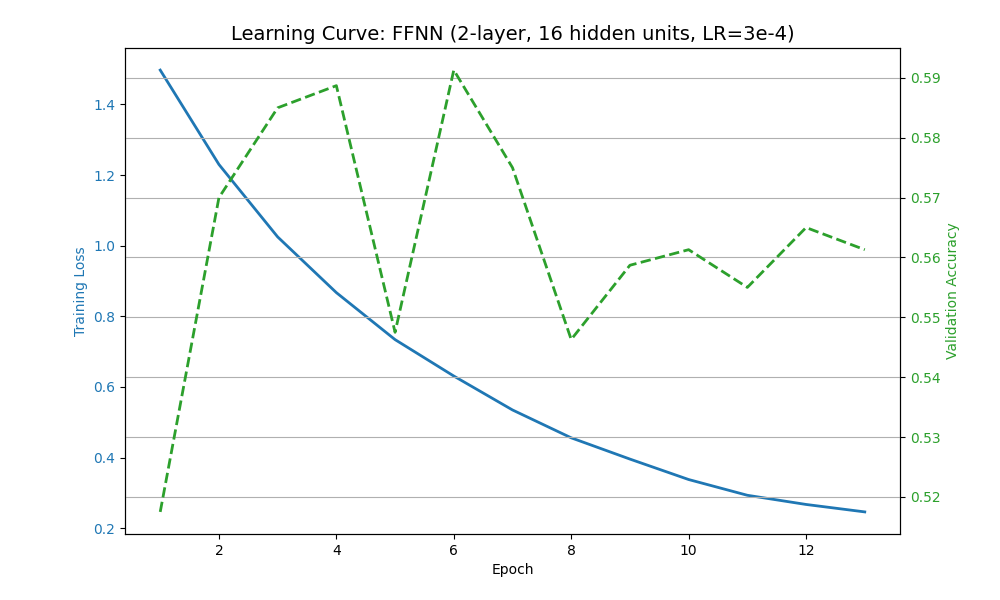
\includegraphics[width=0.8\textwidth]{figs/best-ffnn-plot.png}
    \caption{Learning curve for FFNN (2-layer, 16 hidden units, LR = 3e-4).}
    \label{fig:ffnn-curve}
\end{figure}

\begin{figure}[H]
    \centering
    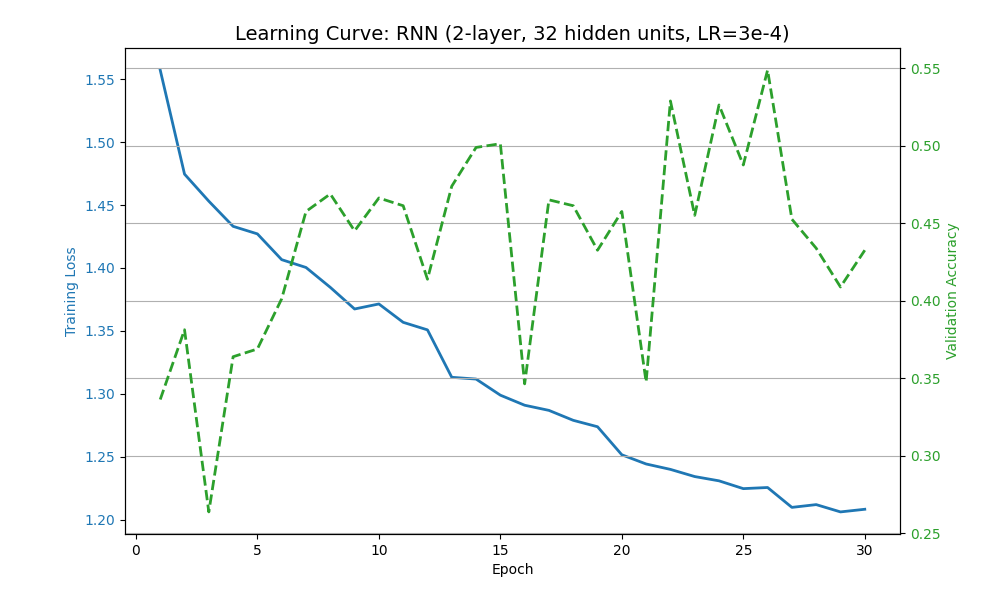
\includegraphics[width=0.8\textwidth]{figs/best-rnn-plot.png}
    \caption{Learning curve for RNN (2-layer, 32 hidden units, LR = 3e-4).}
    \label{fig:rnn-curve}
\end{figure}


\subsection*{Learning Curve}
The learning curve of our best-performing models shows distinct behaviors for the FFNN and the RNN. For the FFNN (with 2 hidden layers and 16 hidden units, LR = 3e-4), the training loss steadily decreases, and the validation accuracy plateaus around epoch 10, after which early stopping was triggered. This indicates stable training and good generalization without overfitting.

On the other hand, the RNN (with 2 layers and 32 hidden units, LR = 3e-4) exhibits a more erratic learning curve, with some fluctuations in both training loss and validation accuracy. These fluctuations suggest that the RNN had some instability during training, which may have contributed to lower validation accuracy, but it still showed improvement over time, indicating the model was learning meaningful patterns despite the noise.


\subsection*{Error Analysis}
One common error observed was the misclassification of ambiguous or out-of-distribution inputs, especially for rare or noisy tokens. RNNs tended to make more inconsistent predictions, likely due to unstable training. In contrast, FFNNs handled consistent patterns better but struggled with long-range dependencies. Improving the feature representation (e.g., using pre-trained embeddings) or applying more regularization could help reduce such errors.


\section{Conclusion and Feedback}


\subsection*{Conclusion}
Our experiments demonstrated that FFNN models outperformed RNNs on this classification task, achieving higher and more consistent validation accuracy. In particular, FFNNs with two hidden layers and smaller hidden dimensions (e.g., 16 or 32) combined with a learning rate of 3e-4 yielded the best results. RNN models showed lower performance and were more sensitive to hyperparameter choices, often struggling with underfitting. Overall, FFNNs provided a more reliable architecture under the tested conditions.


\subsection*{Feedback}
The assignment was engaging and helped reinforce our understanding of model training, tuning, and evaluation. However, it was quite time-consuming, taking approximately 20–25 hours in total. The tuning process—particularly for RNNs—was challenging due to long training times and unstable convergence. It might be helpful to provide a clearer guide or tighter constraints on the hyperparameter search space. Overall, though, the assignment was valuable and realistic, offering practical insight into how models behave under different settings.


\end{document}
